Support Vector Machines are supervised maximum margin models that are used for problems 
such as:
\begin{itemize}
    \item Classification
    \item Regression
    \item Distribution Estimation
\end{itemize}
They are considered supervised because they need a pre-labeled training set to develop 
the hyperplanes that separate the classes. The terminology maximum margin refers to the
fact that the SVM tries to solve a convex optimization problem which maximizes the 
distance between the hyperplane and the closest data points from each class. This 
distance is called "margin".

\begin{figure}[H]
    \centering
    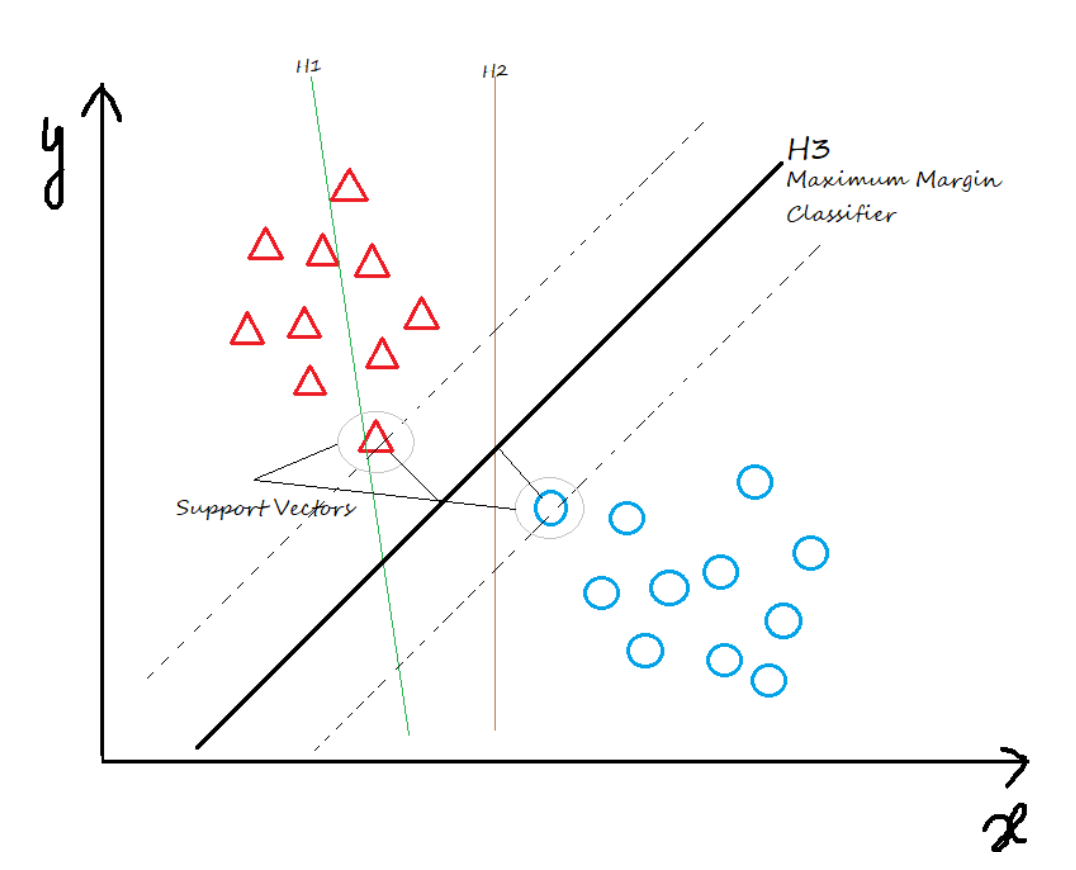
\includegraphics[width=0.5\textwidth]{media/svm_example.png}
    \caption{SVM Maximum Margin Classifier}
\end{figure}
